\documentclass[12pt]{CSUNthesis}
%%%%%%%%%
\textheight=22cm
\def\T{\mathbb{T}}
\def\twotop#1#2{\genfrac{}{}{0pt}{}{#1}{#2}}
% % %
\def\R{\mathbb{R}}
% % % 

%%%%%%%%%
\usepackage{color}
\newcommand{\hl}[1]{\colorbox{lightgray}{#1}}
%\usepackage{tocloft}
\usepackage{setspace}
\usepackage{amsmath}
\usepackage{amssymb}
\usepackage{graphicx}
%\usepackage{subfigure}
%\usepackage{epsfig}
\usepackage{epstopdf}
\usepackage{hyphenat}
\usepackage{setspace}
\usepackage{pdfsync}
\usepackage{tensor}
\usepackage{float}
\usepackage{subfig}
\restylefloat{table}

\setlength{\topmargin}{-0.25in}
\setlength{\textheight}{9.0in}
\setlength{\oddsidemargin}{0.5in} \setlength{\evensidemargin}{0.0in}
\setlength{\textwidth}{6.0in}

\newtheorem{example}{Example}
\newtheorem{theorem}{Theorem}
\newtheorem{proposition}{Proposition}
\newtheorem{corollary}[theorem]{Corollary}
\newtheorem{claim}[theorem]{Claim}
\newtheorem{definition}{Definition}
\newtheorem{remark}{Remark}[section]
\newtheorem{lemma}{Lemma}
\newtheorem{defn}{Definition}[section]

\newtheorem{rem}{Remark}[section]
\newenvironment{proof}[1][Proof]{\noindent\textbf{#1.} }{\newline \hspace*{\textwidth}\hspace*{-0,4cm} \rule{0.5em}{0.5em} \vspace{0,2cm}}

\renewcommand{\baselinestretch}{2}
\newcommand{\Rn}{$\mathbb{R}^n$}
\newcommand{\Rm}{$\mathbb{R}^m$}
\newcommand{\Rns}{$\mathbb{R}^n $ }
\newcommand{\Rnn}{$\mathbb{R}^{n+1}$}
\newcommand{\tb}{\textcolor{blue}}
\newcommand{\tr}{\textcolor{red}}
\newcommand{\D}{\mathrm{d}} % this defines a new command for making the d's in integrals look good
\newcommand{\limit}[3]{\underset{#1 \to #2}{\lim}  #3}  %this defines a command called limit with 3 slots
\newcommand{\manM}{$\mathcal{M}$}
\newcommand{\manMs}{$\mathcal{M} $ }
% Math mode friendly shortcuts
% % %
\def\T{\mathbb{T}}
\def\R{\mathbb{R}}
\def\Sbb{\mathbb{S}}
\def\e{\mathrm{e}}
\def\calF{\mathcal{F}}
\newcommand{\dydx}[2]{\frac{\partial{#1}}{\partial{#2}}}
\newcommand{\vecx}{\vec{x}}
\newcommand{\vecv}{\vec{v}}
\newcommand{\bulkv}{\vec{\bar{v}}} %bulk velocity


\newenvironment{Proof}[1][Proof]{\noindent\textbf{#1.} }{\newline \hspace*{\textwidth}\hspace*{-0,4cm} \rule{0.5em}{0.5em} \vspace{0,2cm}}
%%%%%%%%%

%% ADDITIONAL COMMANDS BEGIN


%%USE TIKPICTURE
\usepackage{tikz}
\usetikzlibrary{fit}
\usetikzlibrary{shapes}
\usetikzlibrary{arrows}
\usetikzlibrary{decorations.markings}
\usetikzlibrary{positioning}

\tikzset{mylabel/.style={font=\footnotesize}}
\tikzset{mymidlabel/.style={fill=white}}
%\tikzset{mymidlabel/.style={fill=white,font=\footnotesize}}

\definecolor{mydark}{RGB}{73,68,62}%{128,129,135}
\definecolor{mymedium}{RGB}{128,129,135}%{167,170,171}
\definecolor{mylight}{RGB}{226,226,226}
\definecolor{myyellow}{RGB}{251,214,0}
\definecolor{mydarkyellow}{RGB}{255,204,13}
%%%%%%%%%%%%%%%%%%%%%%%%%%%%%

\usepackage{lmodern}
\usepackage{mathtools}
\linespread{1.0}
\usepackage[font={small,it}]{caption}
\usepackage{tabularx}
\usepackage{sidecap}
\usepackage{colortbl,xcolor}

\usepackage{algorithm,algpseudocode}


% % % Additional Commands End

%%%%%%%%%

% Set the path to graphics.
\graphicspath{{images/}}

\submitted{August}{2015}

\author{Jeffrey Limbacher}

\title{Working title}

\committee {Alexander Alekseenko , Ph.D.}
		   {Ali Zakeri , Ph.D.}
           {Vladislav Panferov , Ph.D.}

\abstract{tbd}

%\copyrightyear{2015}

\acknowledgement{tbd}

\begin{document}
\doublespacing

%%%%%%%%%%%%%%%%%%%%%%%%%%%%%%%%%%%%%%%%%%%%%%%%%%%%%%%%%
%%%% CHAPTER ONE
%%%%%%%%%%%%%%%%%%%%%%%%%%%%%%%%%%%%%%%%%%%%%%%%%%%%%%%%%

\chapter{Introduction}
\label{Chap1}

%%%%%%%%%%%%%%%%%%%%%%%%%%%%%%%%%%%%%%%%%%%%%%%%%%%%%%%%%
%%%% CHAPTER TWO
%%%%%%%%%%%%%%%%%%%%%%%%%%%%%%%%%%%%%%%%%%%%%%%%%%%%%%%%%

\chapter{The Boltzmann Equation}
\label{Chap2}
	The kinematic theory of gases treats gases as composed of a large number of individual molecules that for large periods of time flow freely. As these particles move freely through space, they collide with each other. Collisions of these particles are what drive the evolution of the gas towards equilibrium. 
	
\section{Binary Collisions of Particles}
\label{sec:bincol}
	This section considers the properties of two particles on a collision path with each other as illustrated in Figure \ref{fig:binary_collision}. In all the work that follows, is is assumed that the molecules undergo elastic hard sphere collisions. 
\begin{figure}[h]
	\centering
	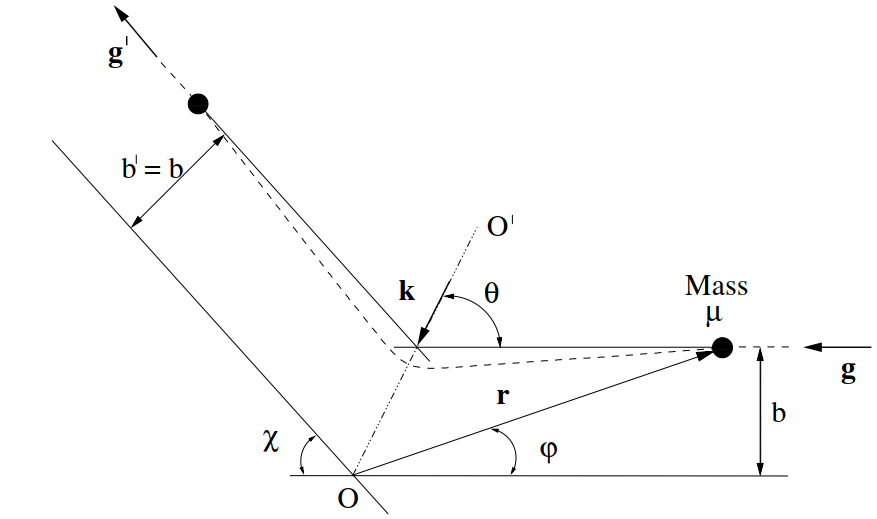
\includegraphics[scale=.5]{binary_collision}
	\caption{Kremer (2010, p. 27), Fig 1.6}
	\label{fig:binary_collision}
\end{figure}
	
	 Denote the pre- and post-collisional asymptotic velocities by $\vec{v}$, $\vec{v_1}$ and $\vec{v}'$, $\vec{v}_1'$ respectively. Define the relative pre- and post-collisional velocities, respectively, by 
\begin{equation*}
	\vec{g} = v_1 - v\, , \quad \vec{g}' = \vec{v}'-\vec{v}_1' \, .
\end{equation*}
$b$ denotes the offset of the centers of the molcules orthogonal to $\vec{g}$. $\varepsilon$ denotes the azimuthal angle between the two particles. 

By conservation of momentum, we have that 
\begin{equation}
\label{eq:consv_momentum}
m \vecv + m \vecv_1 = m\vecv' + m\vecv_1'\, .
\end{equation}
Equation \ref{eq:consv_momentum} yields $|g'| = |g|$. In addition, due to the hard sphere assumption, the collision is considered to be perfectly elastic, giving
\begin{equation}
\label{eq:consv_kin}
\frac{1}{2} m|\vecv| + \frac{1}{2} m|\vecv_1| = \frac{1}{2}m|\vecv'| + \frac{1}{2}m|\vecv_1'|
\end{equation}

The apsidal vector, $\vec{k}$ given by
\begin{equation*}
\vec{k} = \frac{\vec{g} - \vec{g}'}{|\vec{g} - \vec{g'}|}\, ,
\end{equation*}
bisects the angle between asymptotic relative velocities. Using this vector, we can write a relationship between the pre- and post-collisional velocities by
\begin{equation}
\label{eq:vel_relation}
\vec{v}_1' = \vec{v}_1 - \vec{k}(\vec{k} \cdot \vec{g})\, , \quad \vec{v}' = \vec{v} + \vec{k}(\vec{k} \cdot \vec{g})\, .
\end{equation}


\section{The Boltzmann Equation}

We consider a gas enclosed in a volume. A single molecule of this gas can be described with having position $\vec{x}$ and velocity $\vec{v}$ at a time $t$. For a particular time, we can describe a molecule as being within at a single point, $(\vec{x},\vec{v})$, in 6-dmensional space known as phase space. We define the distribution function of the gas as $f(t,\vec{x},\vec{v})d\vec{x}\,d\vec{v}$ gives the number of particles within the range of $\vec{x} + d\vec{x}$ with velocities $\vec{v} + d\vec{v}$. 

In 1872 Boltzmann \cite{Boltzmann1872} introduced the Boltzmann equation which describes the time evolution of the distribution $f$. In the absence of external forces and we ignore collisions of particles, then the Boltzmann equation takes the form
\begin{equation}
\label{eq:colless_boltzmann}
\dydx{}{t}f(t, \vecx, \vecv) + \vecv \cdot \nabla_x f(t, \vecx, \vecv) = 0\, .
\end{equation}
However, when the effects of collisions cannot be neglected, the right hand side must be modified to take this into account. In this case, the Boltzmann equation takes the form of
\begin{equation}
\label{eq:boltzmann}
\dydx{}{t}f(t, \vecx, \vecv) + \vecv \cdot \nabla_x f(t, \vecx, \vecv) = I[f](t,\vecx,\vecv)\, \\ 
\end{equation}
Where $I[f]$ is referred to as the collision operator. The explicit form of $I[f]$ depends on the properties of the gas. To describe it explicitly, we make several assumptions. First, the gas composed entirely of a single species of molecule. Second, we assume hard sphere collisions as described in section \ref{sec:bincol}. 

In order to explicitly write the collision operator, we must describe the collisions within the gas. Consider a particle with velocity $\vecv$. In the volume element $\vecx d\vecx$
\begin{equation}
dt \int_{\R^3} \int_0^{b^*} \int_0^{2\pi} f_1 f b |g|\,  db \, d\varepsilon\, dv_1 \, dv \, .
\end{equation}

\begin{equation}
\label{eq:explicit_I}
I[f](t, \vecx, \vecv) = \int_{\R^3} \int_{\R^3} (f_1' f' - f_1 f) |g|\, b\, db\, d\varepsilon\, d\vecv_1\, ,
\end{equation}
where,
\begin{equation*}
f_1' \equiv f(t, \vecx, \vecv_1')\quad f' \equiv f(t, \vecx, \vecv') \quad f_1 \equiv f(t, \vecx, \vecv_1 \quad f \equiv f(t, \vecx, \vecv)\, .
\end{equation*}
From here, we can substitute (\ref{eq:explicit_I}) into (\ref{eq:boltzmann}) to arrive to the explicit form of the Boltzmann equation,
\begin{equation}
\dydx{}{t}f(t, \vecx, \vecv) + \vecv \cdot \nabla_x f(t, \vecx, \vecv) = \int_{\R^3} \int_{\R^3} (f_1' f' - f_1 f) |g|\, b\, db\, d\varepsilon\, d\vecv_1\, .
\end{equation}
The Boltzmann equation is a non-linear integro-differential equation. The right hand side is a five dimensional integral that must be evaluated at each point in 6-dimensional space.

\section{Moments of the Distribution Function}

A gas is usually described by its macroscopic states. Kinetic theory defines these macroscopic properties in terms of distribution function $f(t,\vecx, \vecv)$. The first five moments of the gas are defined below.
\begin{align}
	n(t,\vec{x})&=\int_{\mathbb{R}^3}  f(t,\vec{x},\vec{v}) d\vec{v} &\text{- number density}  \label{eq:dens} \\
	\bar{v}_i(t,\vec{x})&=\frac{1}{n(t,\vec{x})} \int_{\mathbb{R}^3} m v_i f(t,\vec{x},\vec{v}) d\vec{v} &\text{- bulk velocity} \label{eq:bulk} \\
	T(t,\vec{x}) &= \frac{1}{3Rn(t,\vecx)}\int_{\mathbb{R}^3} m C^2 f(t,\vec{x},\vec{v}) d\vec{v} &\text{- temperature} \label{eq:temperature}
\end{align}
where $C_i=v_i-\bar{v}_i$, $C^2=C_1^2 + C_2^2 + C_3^2$, and $R$ is the specific gas constant. The number density $n(t, \vecx)$ denote the number of particles contained in our distribution. $\bulkv (t,\vecx)$ denotes that average velocity of particles within the gas. The temperature denotes the deviation form the average. 

An important property of the collision integral 

\section{The Maxwellian Distribution}

If the gas is free from external influence, then the gas will approach an equilibrium. In this equilibrium, the gas distribution takes a specific shape known as the Maxwellian distribution given below.
\begin{equation}
f_M(\vec{v},n,\vec{\bar{v}},T) = \frac{1}{\sqrt{2 \pi R T}^3} \exp\left( -\frac{ |\vec{v} - \vec{\bar{v}}|^2}{2RT} \right)
\end{equation} 
	
Note that the exact shape of the Maxwellian distribution depends on the macroscopic moments of the gas distribution, $n$, $\vec{\bar{v}}$, and $T$ given by equations \ref{eq:dens}, \ref{eq:bulk}, \ref{eq:temperature} respectively. This is illustrated in Figure \ref{fig:1d_maxwellian}. The distribution is centered around $\bulkv$. The temperature, $T$, controls the width of the distribution. $n$ determines the area under the curve.
\begin{figure}[h]
\centering
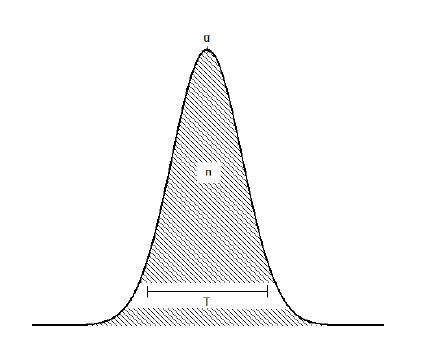
\includegraphics[scale=.5]{1D_Maxwellian}
\caption{Stolen picture need better caption}
\label{fig:1d_maxwellian}
\end{figure}

When the gas is in equilibrium, the difference between the number of particles that enter and leave a particular phase volume vanishes. In other words, 
\begin{equation*}
I[f_M](t,\vecx,\vecv) = \int_{\R^3} \int_{\R^3} f_{M1}'f_M' - f_{M1} f_M  g\, b\, db\, d\varepsilon\, d\vecv_1\ = 0
\end{equation*}

\section{Dimensionless Reduction}

%%%%%%%%%%%%%%%%%%%%%%%%%%%%%%%%%%%%%%%%%%%%%%%%%%%%%%%%%
%%%% CHAPTER THREE
%%%%%%%%%%%%%%%%%%%%%%%%%%%%%%%%%%%%%%%%%%%%%%%%%%%%%%%%%

\chapter{Discontinuous Galerkin Discretization in the Velocity Variable}

Discontinuous Galerkin methods is a method of discretizing equations. The following section describes the DG formulation found in~\cite{AlekseenkoJosyula2012},~\cite{AlekseenkoNguyenWood2015}.

\section{DG Discretization in Velocity Space}
We denote the points in the velocity space as $\vec{v} = (u,v,w)$. The velocity space is reduced to a rectangular parallelpiped $K=[u_L, u_R] \times [v_L,v_R] \times [w_L,w_R]$. It is assumed that outside the parallelpiped the contribution of the function to the first few moments is negligible. Depending on the parallelpiped, this will not result in large errors in terms of conservation of density and temperature. 

We partition $K$ into $N$ smaller rectangular parallelpipeds $K_j = [u_L^j, u_R^j] \times [v_L^j, v_R^j] \times [w_L^j, w_R^j]$. Each $K_j$ will contain a set of basis function, $\phi_j^i$, $i=1,\dots, s$ as described. We introduce nodes of Gauss quadratures of order $s_u$, $s_v$, and $s_w$ on each of the intervals $[u_L^j,u_R^j]$, $[v_L^j,v_R^j]$, and $[w_L^j,w_R^j]$. The nodes are denoted as
$\kappa^{u}_{p;j}$, $\dots$, $p=1,s_{u}$,
$\kappa^{v}_{q;j}$, $\dots$, $q=1,s_{v}$, and 
$\kappa^{w}_{r;j}$, $\dots$, $r=1,s_{w}$. From the nodes, the one-dimensional Lagrange basis functions are defined:
\begin{equation}
\label{eq:01}
\phi^{u}_{l;j}(u)=\prod_{{p=1,s_{u}} \atop {p\neq l}} \frac{\kappa^{u}_{p;j}-u}{\kappa^{u}_{p;j}-\kappa^{u}_{l;j}}\, ,\quad 
\phi^{v}_{m;j}(v)=\prod_{{q=1,s_{v}} \atop {q\neq m}} \frac{\kappa^{v}_{q;j}-v}{\kappa^{v}_{q;j}-\kappa^{v}_{m;j}}\, ,\quad 
\phi^{w}_{n;j}(w)=\prod_{{r=1,s_{w}} \atop {r\neq n}} \frac{\kappa^{w}_{r;j}-w}{\kappa^{w}_{r;j}-\kappa^{w}_{n;j}}\, .
\end{equation}
The three-dimensional basis function is defined as
\begin{equation}
\label{eq:01a}
\phi_{i;j}(\vec{v})=\phi^{u}_{l;j}(u)\phi^{v}_{m;j}(v)
\phi^{w}_{n;j}(w)
\end{equation} 
where $i=1,\dots, s= s_u s_v s_w$. A useful property of the basis functions (\ref{eq:01a}) is that they vanish on all nodes except one. In addition, the quadrature nodes used are exact on polynomials of degree at most $2s_u-1$, $2s_v-1$, and $2s_w-1$. In addition, the following lemma holds,
\begin{lemma} (see also \cite{AlekseenkoJosyula2012a, HesthavenWarburtoin2007})
The following identities hold for basis functions $\phi_{i;j}(\vec{v})$:
\begin{equation}
\label{eq:lemma2.1} 
\int_{K_{j}} \phi_{p;j}(\vec{v})\phi_{q;j}(\vec{v})\, d\vec{v} = \frac{\omega_{p}\Delta\vec{v}^{j}}{8}\delta_{pq}
\qquad\mbox{and} \qquad
\int_{K_{j}} \vec{v}\phi_{p;j}(\vec{v})\phi_{q;j}(\vec{v})\, d\vec{v} 
= \frac{\omega_{p}\Delta\vec{v}^{j}}{8}\vec{v}_{p;j}\delta_{pq},
\end{equation}
where indices $l$, $n$, and $m$ of one dimensional basis functions correspond to 
the three-dimensional basis functions 
$\phi_{p;j}(\vec{v})=
\phi^{u}_{l;j}(u)\phi^{v}_{m;j}(v)\phi^{w}_{n;j}(w)$, 
and the vector $\vec{v}_{p;j}=(\kappa^{u}_{l;j},\kappa^{v}_{m;j},\kappa^{w}_{n;j})$. 
\end{lemma}
\section{Nodal-DG Velocity Discretization of the Boltzmann Equation}
We assume that on each $K_j$, the solution to the Boltzmann equation is sought of the form 
\begin{equation}
\label{eq:3.4}
f(t,\vec{x},\vec{v})|_{K_{j}} = \sum_{i=1,s} f_{i;j}(t,\vec{x})\phi_{i;j}(\vec{v})\, .
\end{equation}
We substitute equation \ref{eq:3.4} into $\ref{eq:boltzmann}$, multiply the result by test basis function, integrate over $K_j$, and apply identity (\ref{eq:lemma2.1}) to arrive to
\begin{equation}
\label{discveloblzm}
\partial_{t} f_{i;j}(t,\vec{x}) + \vec{v}_{i;j}\cdot \nabla_{x} f_{i;j}(t,\vec{x}) =
\frac{8}{\omega_{i}\Delta\vec{v}^{j}}I_{\phi_{i;j}}\, ,
\end{equation}
where $I_{\phi_{i;j}}$ is the projection of the collision operator 
on the basis function $\phi_{i;j}(\vec{v})$:
\begin{equation}
\label{eq:projcoll}
I_{\phi_{i;j}} = \int_{K_{j}}\phi_{i;j}(\vec{v}) I[f](t,\vec{x},\vec{v})\, d\vec{v}\, .
\end{equation} 

\section{Reformulation of the Galerkin Projection of the Collision Operator}
\label{sec:reform_galerkin}
Similarly to \cite{AlekseenkoJosyula2012,AlekseenkoJosyula2012a,Majorana2011}, we rewrite the 
DG projection of the collision operator $I_{\phi_{i;j}}$ in the form of a bilinear integral operator 
with a time-independent kernel. The principles of kinetic theory suggest that changes to $f(t,\vecx, \vecv)$ with respect to $\vecx$ at the distance of a few $b^*$ are negligible, see e.g., \cite{Struchtrup2005}. Specifically, using the well-known identities (see, e.g.,  \cite{Kogan1969}, Section 2.4), and applying the first principles assumption, we have 
\begin{align}
\label{eq:transfer_eq}
I_{\phi_{i;j}}&= \int_{\R^3}\int_{\R^3} f(t,\vec{x},\vec{v}) f(t,\vec{x},\vec{v}_{1})
\int_{\Sbb^2}(\phi_{i;j}(\vec{v}')-\phi_{i;j}(\vec{v})) b_{\alpha}(\theta) |g|^\alpha \, d\sigma\,
 d\vec{v}_{1}\, d\vec{v} \nonumber \\
{} & = \int_{\R^3}\int_{\R^3} f(t,\vec{x},\vec{v}) f(t,\vec{x},\vec{v}_{1})
 A(\vec{v},\vec{v}_{1};\phi_{i;j})   d\vec{v}_{1}\, d\vec{v}\, ,
\end{align}
where  
\begin{align}
\label{eq:A_definition}
A(\vec{v},\vec{v}_{1};\phi_{i;j})= |g|^\alpha \int_{\Sbb^2} (\phi_{i;j}(\vec{v}')
- \phi_{i;j}(\vec{v})) b_{\alpha}(\theta) \, d\sigma\, .
\end{align}
The kernel $A(\vec{v},\vec{v}_{1};\phi_{i;j})$ is independent of time and can be pre-computed. 
In \cite{AlekseenkoJosyula2012a} properties of a kernel closely related to $A(\vec{v},\vec{v}_{1};\phi_{i;j})$ 
are considered.
In particular, due to the local support of $\phi_{i;j}(\vec{v})$, it is anticipated that 
kernel  $A(\vec{v},\vec{v}_{1};\phi_{i;j})$ will have only $O(M^{5})$ non-zero components for each $\phi_{i;j}(\vec{v})$, 
where $M$ is the number of discrete velocity points in each velocity dimension. As a result, evaluation of  
(\ref{eq:transfer_eq}) will require $O(M^{8})$ operations for each spatial point. This number of evaluations 
is very high. However, as we will show later, it can be reduced to $O(M^6)$ operations using symmetries of
$A(\vec{v},\vec{v}_{1};\phi_{i;j})$, the convolution form of (\ref{eq:transfer_eq}) and the Fourier 
transform. 

We remark that in many numerical re-formulations of the Boltzmann equation, the collision 
operator is separated into the gain and loss terms.
This separation can be performed in (\ref{eq:transfer_eq}),
\begin{align}
I_{\phi_{i;j}}&= \int_{\R^3}\int_{\R^3} f(t,\vec{x},\vec{v}) f(t,\vec{x},\vec{v}_{1})
\int_{\Sbb^2}(\phi_{i;j}(\vec{v}')-\phi_{i;j}(\vec{v})) b_{\alpha}(\theta) |g|^\alpha \, d\sigma\,
 d\vec{v}_{1}\, d\vec{v} \nonumber \\
&= \int_{\R^3}\int_{\R^3} f(t,\vec{x},\vec{v}) f(t,\vec{x},\vec{v}_{1}) (\int_{\Sbb^2}\phi_{i;j}(\vec{v}')b_{\alpha}(\theta) |g|^\alpha d\sigma\, - |g|^\alpha\int_{\Sbb^2}\phi_{i;j}(\vec{v})b_{\alpha}(\theta)  d\sigma\,)  d\vec{v}_{1}\, d\vec{v} \nonumber \\
&= \int_{\R^3}\int_{\R^3} f(t,\vec{x},\vec{v}) f(t,\vec{x},\vec{v}_{1}) (A^+(\vecv,\vecv_1;\phi_{i;j}) - |g|^\alpha \sigma_T)  d\vec{v}_{1}\, d\vec{v}
\end{align}
where
\begin{equation}
A^+(\vecv,\vecv_1;\phi_{i;j}) = \int_{\Sbb^2}\phi_{i;j}(\vec{v}')b_{\alpha}(\theta) |g|^\alpha d\sigma\, , \quad \sigma_T = \int_{\Sbb^2}\phi_{i;j}(\vec{v})b_{\alpha}(\theta)  d\sigma\, .
\end{equation}
Theoretical properties of $A^+(\vecv,\vecv_1;\phi_{i;j}$ are very similar to that of $A(\vecv,\vecv_1;\phi_{i;j})$. 
$A^+(\vecv,\vecv_1;\phi_{i;j})$ has theoretical properties that are better than that of $A(\vecv,\vecv_1;\phi_{i;j})$ for a Fourier transform. 
$A(\vecv,\vecv_1;\phi_{i;j})$ is grows linearly to infinity in some direction whereas $A^+(\vecv,\vecv_1;\phi_{i;j})$ does not. It can then be argued that $A^+(\vecv,\vecv_1;\phi_{i;j})$ is better suited for a Fourier transform than $A(\vecv,\vecv_1;\phi_{i;j})$. The algorithms in this paper also have straightforward extensions to the the split formulation of (\ref{eq:transfer_eq}). However, in practice, the split formulation of (\ref{eq:transfer_eq}) had significant errors in conservation.

\section{Properties of the Kernel $A(\vecv,\vecv_1;\phi_{i;j})$}
\label{sec:props_of_a}
\begin{lemma}
\label{lem1} 
Let operator $A(\vec{v},\vec{v}_{1};\phi_{i;j})$ be defined by (\ref{eq:A_definition}). Then $\forall\xi\in \R^3$
\begin{equation*}
A(\vec{v}+\vec{\xi},\vec{v}_{1}+\vec{\xi};\phi_{i;j}(\vec{v}-\vec{\xi}))=
A(\vec{v},\vec{v}_{1};\phi_{i;j}) \, .
\end{equation*}
\end{lemma}

\proof
Consider $A(\vec{v}+\vec{\xi},\vec{v}_{1}+\vec{\xi};\phi_{i;j}(\vec{v}-\vec{\xi}))$. We clarify that these notations mean that
particle velocities $\vec{v}$ and $\vec{v}_{1}$ in (\ref{eq:A_definition}) are replaced with $\vec{v}+\vec{\xi}$ and $\vec{v}_{1}+\vec{\xi}$
correspondingly and that basis function $\phi_{i;j}(\vec{v})$ is replaced with a ``shifted'' function 
$\phi_{i;j}(\vec{v}-\vec{\xi})$. We notice that the relative speed of the molecules with velocities $\vec{v}+\vec{\xi}$ 
and $\vec{v}_{1}+\vec{\xi}$ is still $\vec{g}=\vec{v}+\vec{\xi}-(\vec{v}_{1}+\vec{\xi}_{1})=\vec{v}-\vec{v}_{1}$. 
The post-collision velocities for the pair of particles will be $\vec{v}'+\vec{\xi}$ and $\vec{v}'_{1}+\vec{\xi}$, where $\vec{v}'$ and $\vec{v}'_{1}$ are given by (\ref{eq:vel_relation}). We notice, in particular, that choices of $\theta$ and $\varepsilon$ in 
(\ref{eq:vel_relation}) are not affected by $\vec{\xi}$. The rest of the statement follows by a direct substitution:
\begin{align*}
A(\vec{v}&+\vec{\xi},\vec{v}_{1}+\vec{\xi};\phi_{i;j}(\vec{v}-\vec{\xi})) = |g|^{\alpha} \int_{\Sbb^2} \phi_{i;j}((\vec{v}'+\vec{\xi})-\vec{\xi}) b_{\alpha}(\theta)\, d\sigma\,= |g|^{\alpha} \int_{\Sbb^2} \phi_{i;j}(\vec{v}') b_{\alpha}(\theta)\, d\sigma \\
&  = A(\vec{v},\vec{v}_{1};\phi_{i;j})\, . 
\end{align*}
\endproof
We remark that Lemma~{\ref{lem1}} holds for all potentials of molecular 
interaction used in rarefied gas dynamics. This property was used in 
\cite{AlekseenkoJosyula2012a} to reduce the storage requirement 
on uniform partitions. 

\section{Rewriting the Collision Operator in the Form of a Convolution (Mostly Copy and Pasted from the Paper, needs rewrite?)}
It was shown in~\cite{AlekseenkoNguyenWood2015} that the Galerkin projection of the collision operator can be reformulated in terms of a convolution. This work is recalled in this section. 
We select a partition cell $K_c$ and designate this cell as a generating cell. 
Similarly, the basis functions $\phi_{i;c}(\vec{v})$ on $K_c$ are designated as the generating basis functions. 
Basis functions $\phi_{i;j}(\vec{v})$ on other cells can be obtained using a shift in the velocity variable, namely $\phi_{i;j} (\vec{v})=\phi_{i;c} (\vec{v}+\vec{\xi_{j}})$ where $ \vec{\xi}_{j} \in \mathbb{R}^3$ is the vector that connects the center of $K_j$ to the center of $K_c$.

According to  Lemma~{\ref{lem1}}, operator $A(\vec{v},\vec{v}_1,\phi_{i;j})$ is invariant with respect to translations. Therefore
\begin{align}
\label{eq3.1}
I_{\phi_{i;j}} &= \int_{\R^3}\int_{\R^3} f(t,\vec{x},\vec{v})f(t,\vec{x},\vec{v}_{1})A(\vec{v}+\vec{\xi_{j}},\vec{v}_1+\vec{\xi_{j}}; \phi_{i;j}(\vec{u} - \vec{\xi_{j}})) \, d\vec{v}_{1} d\vec{v} \notag\\
 &= \int_{\R^3}\int_{\R^3} f(t,\vec{x},\vec{v})f(t,\vec{x},\vec{v}_{1})A(\vec{v}+\vec{\xi^{j}},\vec{v}_{1}+\vec{\xi_{j}}; \phi_{i;c}(\vec{u})) \, d\vec{v} d\vec{v_{1}} \, .
\end{align}
Performing the substitutions $\vec{\hat{v}} = \vec{v}+\vec{\xi_{j}} $ and $ \vec{\hat{v}}_1 = \vec{v}_{1}+\vec{\xi_{j}}$ in (\ref{eq3.1}), we have
\begin{equation*}
I_{\phi_{i;j}} = \int_{\R^3}\int_{\R^3} f(t,\vec{x},\vec{\hat{v}}-\vec{\xi_{j}}) f(t,\vec{x},\vec{\hat{v}}_1-\vec{\xi_{j}}) A(\vec{\hat{v}},\vec{\hat{v}}_{1};\phi_{i;c}(\vec{u})) \, d\vec{\hat{v}} d\vec{\hat{v}}_1 \, .
\end{equation*}
We then introduce a bilinear convolution operator, $i=1,\ldots,s$
\begin{equation}
\label{eq:continuous_convolution}
I_i(\vec{\xi}) = \int_{\R^3}\int_{\R^3} f(t,\vec{x},\vec{v}-\vec{\xi})f(t,\vec{x},\vec{v}_{1}-\vec{\xi})A(\vec{v},\vec{v}_{1}; \phi_{i;c}) \, d\vec{v} d\vec{v}_{1} \, ,
\end{equation}
and notice that $I_{\phi_{i;j}}$ can be obtained from (\ref{eq:continuous_convolution}) as
$I_{\phi_{i;j}}=I_i(\vec{\xi}_j)$. In the following, we will refer to (\ref{eq:continuous_convolution}) 
as the convolution form of the Galerkin projection of the collision integral.

\section{Discretization of the Collision Integral (COpy and pasted again)}
In order to calculate (\ref{eq:continuous_convolution}), we replace the three-dimensional integrals with the Gauss quadratures associated with then nodal-DG discretization, (\ref{eq:01a}). 
As is discussed above, we are only interested in 
computing convolution (\ref{eq:continuous_convolution}) at vectors 
$\vec{\xi}=\vec{\xi}_{j}$ that connect centers of the velocity cells $K_j$ to the 
center of the velocity cell $K_c$, the support of $\phi_{i;c}(\vec{v})$. Since the 
same nodal points are used on all velocity cells, shifts $\vec{\xi}_{j}$ 
translate nodal points in one cell to nodal points 
in another cell. As a result, the quadrature sums to evaluate convolution (\ref{eq:continuous_convolution})
use values of the unknown $f(t,\vec{x},\vec{v})$ at the nodal points
only. In fact, the shift in the velocity variable 
$\vec{v}_{i;l}-\vec{\xi}_{j}$ will correspond 
to a shift in the three dimensional index of the velocity cell 
which we will write formally as $l-j$, 
producing the velocity node $\vec{v}_{i;l-j}(\vec{v})$. The exact expression 
for the shift $l-j$ will be made clear later by considering the cell indices in 
each velocity dimension. The index $i$ of the node within the cell is not 
affected in this process. 

We can write the discrete form of (\ref{eq:continuous_convolution}) as 
\begin{equation}
\label{eq:I_dist}
I_{i;j}:=I_{i}(\vec{\xi}_{j}) = \sum_{i',i''=1}^s  \sum_{j'=1}^{M^3} \sum_{j''=1}^{M^3} f_{i';j'-j} f_{i'';j''-j} A_{i',i'';j',j'';i} 
\end{equation}
where $f_{i';j'-j}=f(t,\vec{x},\vec{v}_{i';j'-j})$, 
$A_{i',i'';j',j'';i}=A(\vec{v}_{i';j'},\vec{v}_{i'';j''}; \phi_{i;c})$ and the three dimensional 
indices $i'$ and $i''$ run over the velocity nodes within a single velocity cell 
and indices $j'$ and $j''$ run over all velocity cells. We note that for some index 
shifts $j'-j$, the resulting cells are outside of the velocity domain. 
In \cite{AlekseenkoJosyula2012a} the values outside of the domain 
were substituted with zeros. In cases when the support of the solution 
was well contained within the computational domain, this assumption did not lead to 
large numerical errors. 

We note that in order to calculate (\ref{eq:I_dist}), it would require $O(M^9)$ operations to calculate it, $O(M^6)$ at one velocity node for $O(M^3)$ velocity nodes. However, recall that the property stated in section \ref{sec:reform_galerkin} that only has $O(M^5)$ components bringing down the total cost of computing (\ref{eq:I_dist}) down to $O(M^8)$ operations. However, we wish to reduce this further. It turns out that the Discrete Fourier Transform has properties that allow us to bring down the cost of computing (\ref{eq:I_dist}) from $O(M^8)$ to $O(M^6)$.

%%%%%%%%%%%%%%%%%%%%%%%%%%%%%%%%%%%%%%%%%%%%%%%%%%%%%%%%%
%%%% CHAPTER FOUR
%%%%%%%%%%%%%%%%%%%%%%%%%%%%%%%%%%%%%%%%%%%%%%%%%%%%%%%%%

\chapter{The Discrete Fourier Transform}

\section{Discrete Convolutions, Circular Convolutions, and Periodic Continuation}




%%%%%%%%%%%%%%%%%%%%%%%%%%%%%%%%%%%%%%%%%%%%%%%%%%%%%%%%%
%%%% CHAPTER FIVE
%%%%%%%%%%%%%%%%%%%%%%%%%%%%%%%%%%%%%%%%%%%%%%%%%%%%%%%%%

\chapter{Discretization of the Collision Integral and Fast Evaluation of Discrete Convolution}

\clearpage
\addcontentsline{toc}{chapter}{References}
\bibliographystyle{plain}
\bibliography{ffb10092017}
\end{document}